\documentclass[12pt, a4paper]{article} %determina o tamanho da fonte, o tipo de papel e o tipo de documento.

\setlength{\parindent}{1.0 cm} %tamanho do espaço para começar o parágrafo.
\setlength{\parskip}{0.5cm} %tamanho do espaço entre os parágrafos.

%Aqui ficam os pacotes utilizados para formatação do documento de modo geral:

\usepackage[utf8]{inputenc} 
\usepackage{indentfirst} %Coloca espaços nos inícios de parágrafos automaticamente. 
\usepackage[brazilian]{babel} %
\usepackage{amsmath}
\usepackage[hmargin=3cm, vmargin=2.5cm, bmargin=2.5cm]{geometry}
\usepackage{multicol}
\usepackage{graphicx} %para poder inserir imagens
\usepackage{subfig}
\usepackage{booktabs} 
\usepackage{hyperref} %para poder adicionar links e hiperlinks
\usepackage{float} %para poder posicionar as imagens


\usepackage{listings} %para poder incluir códigos
\usepackage{xcolor}
\definecolor{codegreen}{rgb}{0,0.6,0}
\definecolor{codegray}{rgb}{0.5,0.5,0.5}
\definecolor{codepurple}{rgb}{0.58,0,0.82}
\definecolor{backcolour}{rgb}{0.95,0.95,0.92}
\lstdefinestyle{mystyle}{
    backgroundcolor=\color{backcolour},   
    commentstyle=\color{codegreen},
    keywordstyle=\color{magenta},
    numberstyle=\tiny\color{codegray},
    stringstyle=\color{codepurple},
    basicstyle=\ttfamily\footnotesize,
    breakatwhitespace=false,         
    breaklines=true,                 
    captionpos=b,                    
    keepspaces=true,                 
    numbers=left,                    
    numbersep=5pt,                  
    showspaces=false,                
    showstringspaces=false,
    showtabs=false,                  
    tabsize=2,
    morecomment={l}[!],
    language=[77]Fortran,
}
\lstset{style=mystyle}

\begin{document} %começa alguma coisa,neste caso, o documento, sempre importante lembrar de colocar o \end{} para não dar erro 
	
	\begin{titlepage}
		\begin{center}
\Huge{Universidade de São Paulo}\\
\large{Instituto de Física de São Carlos}\\
\vspace{20pt}
\vspace{200pt}
\textbf{Lista 2}\\
\vspace{8cm}
		\end{center}

\begin{flushleft}
\begin{tabbing}
Pedro Calligaris Delbem 5255417\\
\end{tabbing}
\vspace{0.5cm}
Professor: Attilio Cucchieri\\		
		\end{flushleft}
	
		\begin{center}
			\vspace{\fill}
	Março de 2025	
		\end{center}
	\end{titlepage}

%####################################################################### SUMÁRIO
	\tableofcontents 
	\thispagestyle{empty}
	\newpage
%#########################################################################

\section{Finding roots}

    \subsection{Exerc\'icio 1}

        Tarefa: Demonstrar que no m\'etodo de Newton-Raphson
        \begin{equation}
            x_{k+1} = x_{k} + \frac{f(x_{k})}{f'(x_{k})}
        \end{equation}
        a converg\^encia \'e quadr\'atica.

        Expandimos f(x) em torno de $x_{n} - r$ - onde r \'e a raiz de f(x) - e obtemos:
        \begin{equation}
            f(x_{n}) = f(r) + f'(r)(x_{n} - r) + \frac{1}{2} f''(r)(x_{n}  - r)^2 + O(x_{n} - r)^3
        \end{equation}
        E como f(r) = 0, obtemos:
        \begin{equation}
            f(x_{n}) = f'(r)(x_{n} - r) + \frac{1}{2} f''(r)(x_{n}  - r)^2 + O(x_{n} - r)^3
        \end{equation}
        Expande-se, também, $f'(x_{n})$ e obtemos:
        \begin{equation}
            f'(x_{n}) = f'(r) + f''(x_{n} - r)(x_{n} - r) + O(x{n} - r)^2
        \end{equation}
        Substituindo em $x_{n+1} = x_{n} + \frac{f(x_{n})}{f'(x_{n})}$ obtemos:
        \begin{equation}
            x_{n+1} = x_{n} - \frac{f'(r)(x_{n} - r) + \frac{1}{2} f''(r)(x_{n}  - r)^2}{f'(r) + f''(x_{n} - r)(x_{n} - r)}
        \end{equation}
        Subtraindo r de ambos os lados:
        \begin{equation}
            x_{n+1} - r = x_{n} - r - \frac{f'(r)(x_{n} - r) + \frac{1}{2} f''(r)(x_{n}  - r)^2}{f'(r) + f''(x_{n} - r)(x_{n} - r)}
        \end{equation}
        Colocando o termo $x_{n} - r$ em evid\^encia:
        \begin{equation}
            x_{n+1} - r = (x_{n} - r)\bigg[1 - \frac{f'(r) + \frac{1}{2} f''(r)(x_{n}  - r)}{f'(r) + f''(x_{n} - r)(x_{n} - r)}\bigg]
        \end{equation}
        Para $x_{n} - r$ pequeno, f''(r)$(x_{n} - r)$ \'e disprez\'ivel e assim o desprezamos no denominador - obtendo:
        \begin{equation}
            x_{n+1} - r = (x_{n} - r)\bigg[1 - \frac{f'(r) + \frac{1}{2} f''(r)(x_{n}  - r)}{f'(r)}\bigg]
        \end{equation}
        Isolando $x_{n} - r$:
        \begin{equation}
            x_{n+1} - r = -(x_{n} - r)^2\bigg[\frac{\frac{1}{2} f''(r)}{f'(r)}\bigg]
        \end{equation}
        Rearranjando:
        \begin{equation}
            r - x_{n+1} = (r - x_{n})^2\bigg[\frac{\frac{1}{2} f''(r)}{f'(r)}\bigg]
        \end{equation}
        Como $r - x_{n}$ \'e o erro cometido na n-\'essima itera\c{c}\~ao e $r - x_{n+1}$ \'e o erro cometido na n+1-\'essima itera\c{c}\~ao, temos que o erro da itera\c{c}\~ao n+1 \'e proporcional ao quadrado do erro da itera\c{c}\~ao n e portanto a converg\^encia \'e quadratica.


%        C\'odigo Escrito:
%        \lstinputlisting[language=Fortran]{../L2-5255417-ex-1.f90}

%        Resultados:
%        \begin{figure}
%            \centering
%            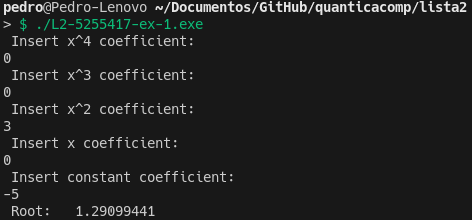
\includegraphics[width=0.8\textwidth]{../images/results-ex-1.png}
%         \caption{Teste feito para gerar o gr\'afico}
%        \end{figure}

%        \begin{figure}[H]
%            \centering
%            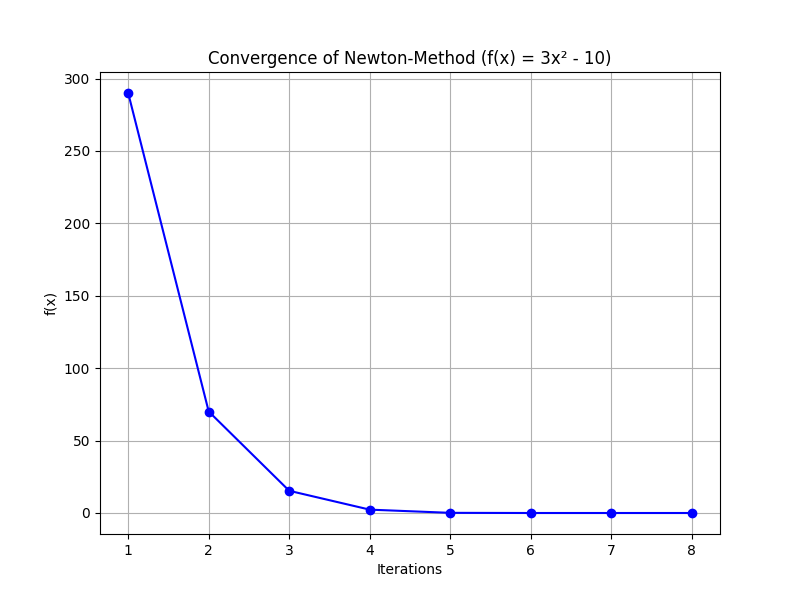
\includegraphics[width=0.8\textwidth]{../images/grafic-ex-1.png}
%            \caption{f(x) ao decorrer das itera\c{c}\~oes}
%        \end{figure}
       
%        Testando para o caso $f(x) = 3x^2 - 10 = 0$ percebe-se  que o m\'etodo Newton-Raphson converge quadraticamente.

    \subsection{Exerc\'icio 2}

        Tarefa: Achar as ra\'zes das equa\c{c}\~oes $f(x) = x^2 - 5 = 0$ e $f(x) = 5x^3 - 5x - 24 = 0$ usando os m\'etodos de Newton-Raphson e da secante para diferentes chutes iniciais e diferentes condi\c{c}\~oes de converg\^encia.

        C\'odigo Escrito:
        \lstinputlisting[language=Fortran]{../L2-5255417-ex-2.f90}

        Resultados:

        \subsubsection{Raizes de $f(x) = x^2 - 5 = 0$}

            Para as seguintes informa\c{c}\~oes iniciais:
            \begin{figure}[H]
                \centering
                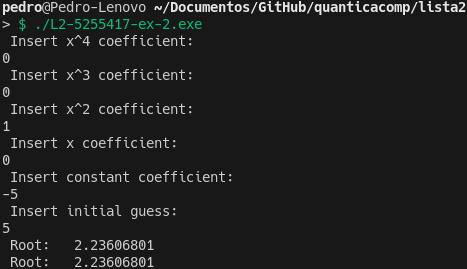
\includegraphics[width=0.8\textwidth]{../images/results-ex-2-5.png}
                \caption{Teste feito para gerar o gr\'afico onde as duas \'ultimas linhas s\~ao as raizes encontradas pelos m\'etodos de Newton-Raphson e da secante, respectivamente}
            \end{figure}
            Obteve-se o valor da raiz = 2.23606801 para ambos os m\'etodos.

            Com o seguinte gr\'afico para o m\'etodo de Newton-Raphson:
            \begin{figure}[H]
                \centering
                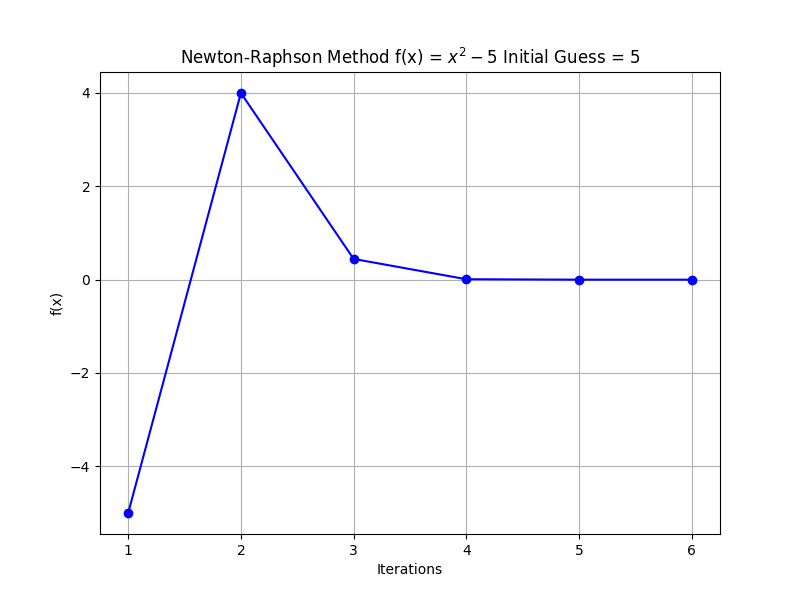
\includegraphics[width=0.8\textwidth]{../images/grafic-ex-2-newton-raphson-method-5.png}
                \caption{f(x) ao decorrer das itera\c{c}\~oes}
            \end{figure}
            Com o seguinte gr\'afico para o m\'etodo da secante:
            \begin{figure}[H]
                \centering
                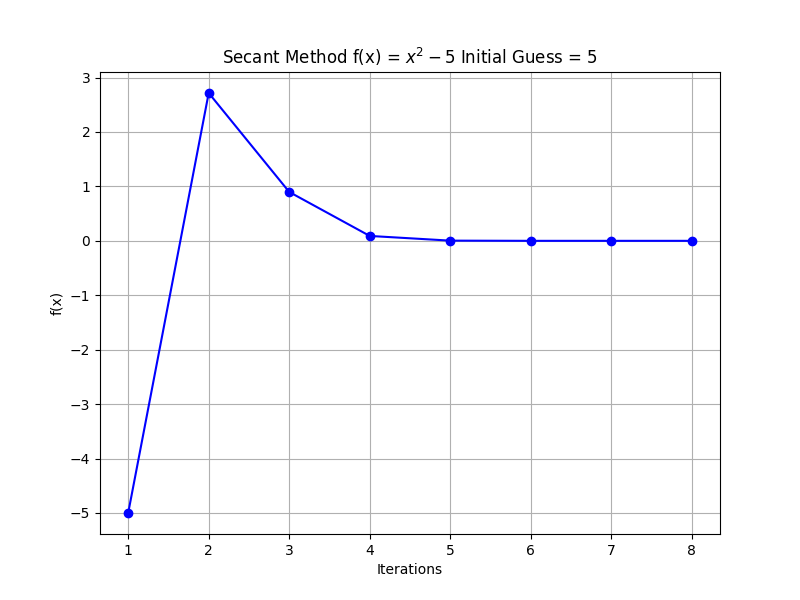
\includegraphics[width=0.8\textwidth]{../images/grafic-ex-2-secant-method-5.png}
                \caption{f(x) ao decorrer das itera\c{c}\~oes}
            \end{figure}

            Para as seguintes informa\c{c}\~oes iniciais:
            \begin{figure}[H]
                \centering
                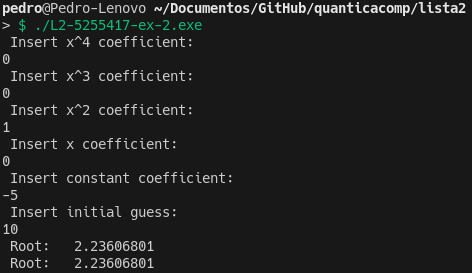
\includegraphics[width=0.8\textwidth]{../images/results-ex-2-10.png}
                \caption{Teste feito para gerar o gr\'afico onde as duas \'ultimas linhas s\~ao as raizes encontradas pelos m\'etodos de Newton-Raphson e da secante, respectivamente}
            \end{figure}
            Obteve-se o valor da raiz = 2.23606801 para ambos os m\'etodos.

            Com o seguinte gr\'afico para o m\'etodo de Newton-Raphson:
            \begin{figure}[H]
                \centering
                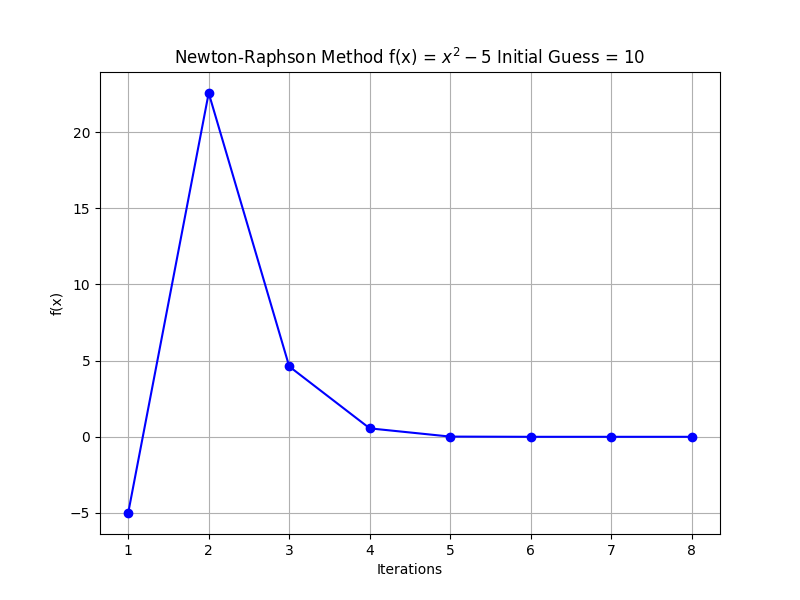
\includegraphics[width=0.8\textwidth]{../images/grafic-ex-2-newton-raphson-method-10.png}
                \caption{f(x) ao decorrer das itera\c{c}\~oes}
            \end{figure}
            Com o seguinte gr\'afico para o m\'etodo da secante:
            \begin{figure}[H]
                \centering
                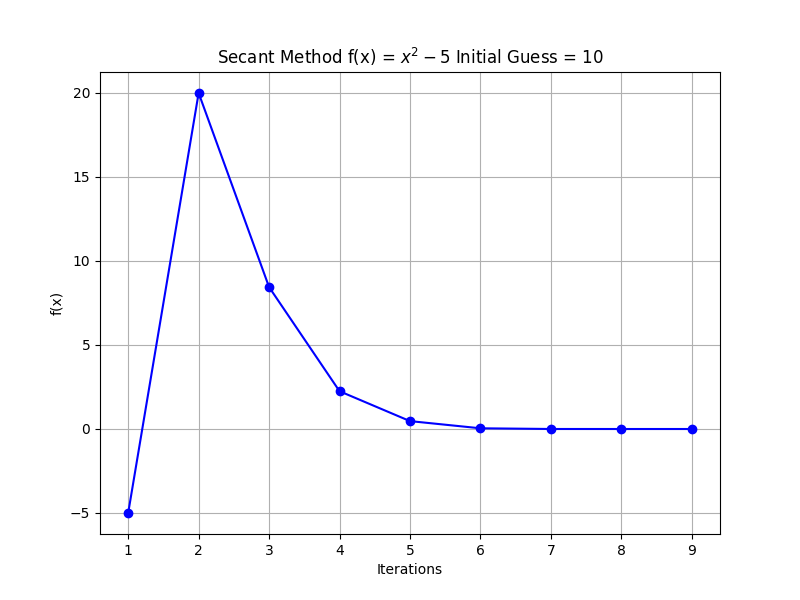
\includegraphics[width=0.8\textwidth]{../images/grafic-ex-2-secant-method-10.png}
                \caption{f(x) ao decorrer das itera\c{c}\~oes}
            \end{figure}

            Para as seguintes informa\c{c}\~oes iniciais:
            \begin{figure}[H]
                \centering
                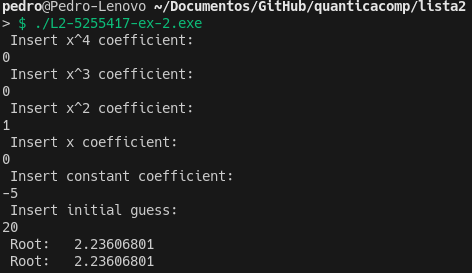
\includegraphics[width=0.8\textwidth]{../images/results-ex-2-20.png}
                \caption{Teste feito para gerar o gr\'afico onde as duas \'ultimas linhas s\~ao as raizes encontradas pelos m\'etodos de Newton-Raphson e da secante, respectivamente}
            \end{figure}
            Obteve-se o valor da raiz = 2.23606801 para ambos os m\'etodos.

            Com o seguinte gr\'afico para o m\'etodo de Newton-Raphson:
            \begin{figure}[H]
                \centering
                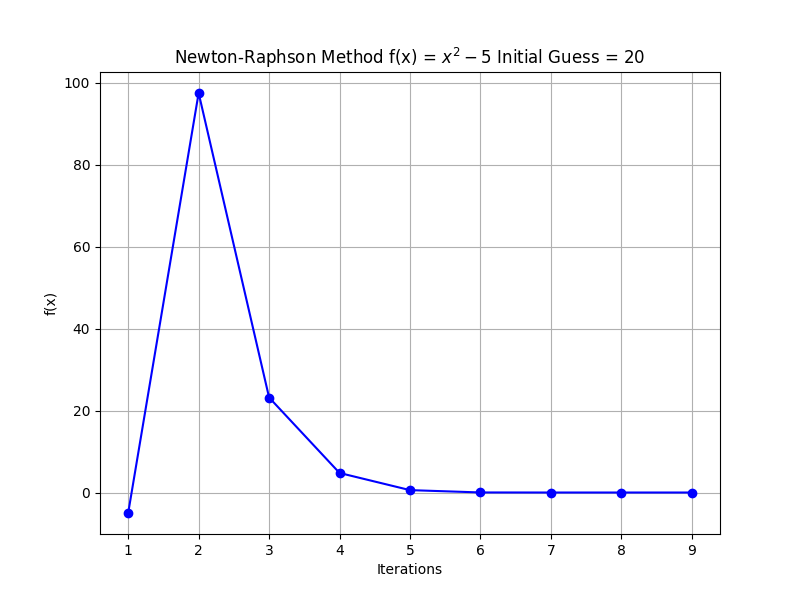
\includegraphics[width=0.8\textwidth]{../images/grafic-ex-2-newton-raphson-method-20.png}
                \caption{f(x) ao decorrer das itera\c{c}\~oes}
            \end{figure}
            Com o seguinte gr\'afico para o m\'etodo da secante:
            \begin{figure}[H]
                \centering
                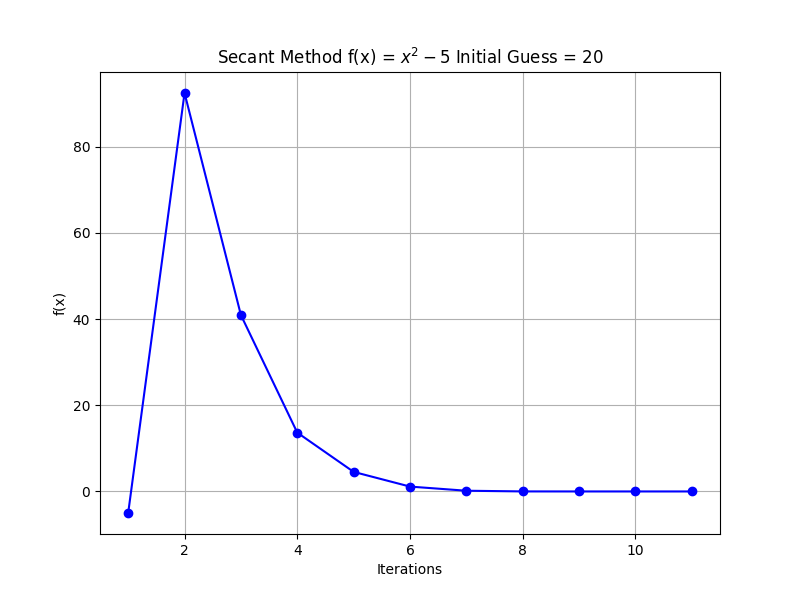
\includegraphics[width=0.8\textwidth]{../images/grafic-ex-2-secant-method-20.png}
                \caption{f(x) ao decorrer das itera\c{c}\~oes}
            \end{figure}

        Percebe-se que ambos os m\'etodos foram suficientes para encontrar as raizes da fun\c{c}\~ao. Contudo o m\'etodo de Newton-Raphson foi mais eficiente em encontrar em menos itera\c{c}\~oes as raizes da fun\c{c}\~ao.

        \subsubsection{Raizes de $f(x) = 5x^3 - 5x - 24 = 0$}
            
            Para as seguintes informa\c{c}\~oes iniciais:
            \begin{figure}[H]
                \centering
                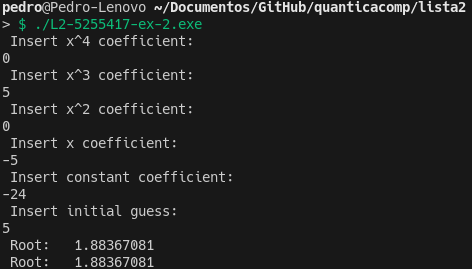
\includegraphics[width=0.8\textwidth]{../images/results-ex-2.2-5.png}
                \caption{Teste feito para gerar o gr\'afico onde as duas \'ultimas linhas s\~ao as raizes encontradas pelos m\'etodos de Newton-Raphson e da secante, respectivamente}
            \end{figure}
            Obteve-se o valor da raiz = 1.88367081 para ambos os m\'etodos.

            Com o seguinte gr\'afico para o m\'etodo de Newton-Raphson:
            \begin{figure}[H]
                \centering
                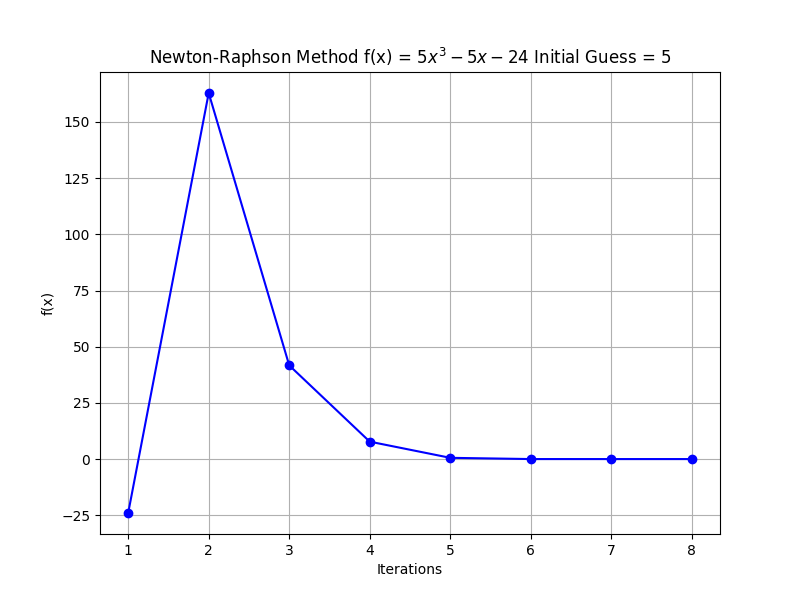
\includegraphics[width=0.8\textwidth]{../images/grafic-ex-2.2-newton-raphson-method-5.png}
                \caption{f(x) ao decorrer das itera\c{c}\~oes}
            \end{figure}
            Com o seguinte gr\'afico para o m\'etodo da secante:
            \begin{figure}[H]
                \centering
                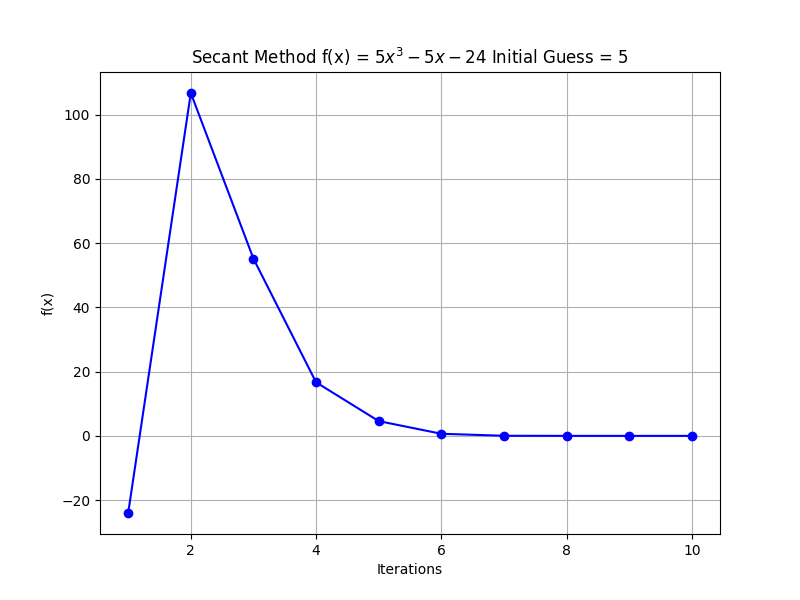
\includegraphics[width=0.8\textwidth]{../images/grafic-ex-2.2-secant-method-5.png}
                \caption{f(x) ao decorrer das itera\c{c}\~oes}
            \end{figure}

            Para as seguintes informa\c{c}\~oes iniciais:
            \begin{figure}[H]
                \centering
                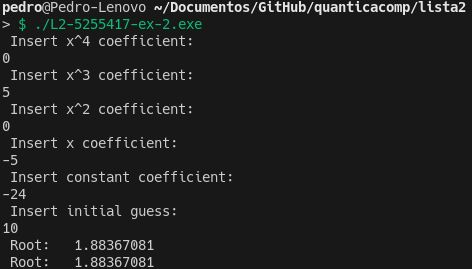
\includegraphics[width=0.8\textwidth]{../images/results-ex-2.2-10.png}
                \caption{Teste feito para gerar o gr\'afico onde as duas \'ultimas linhas s\~ao as raizes encontradas pelos m\'etodos de Newton-Raphson e da secante, respectivamente}
            \end{figure}
            Obteve-se o valor da raiz = 1.88367081 para ambos os m\'etodos.

            Com o seguinte gr\'afico para o m\'etodo de Newton-Raphson:
            \begin{figure}[H]
                \centering
                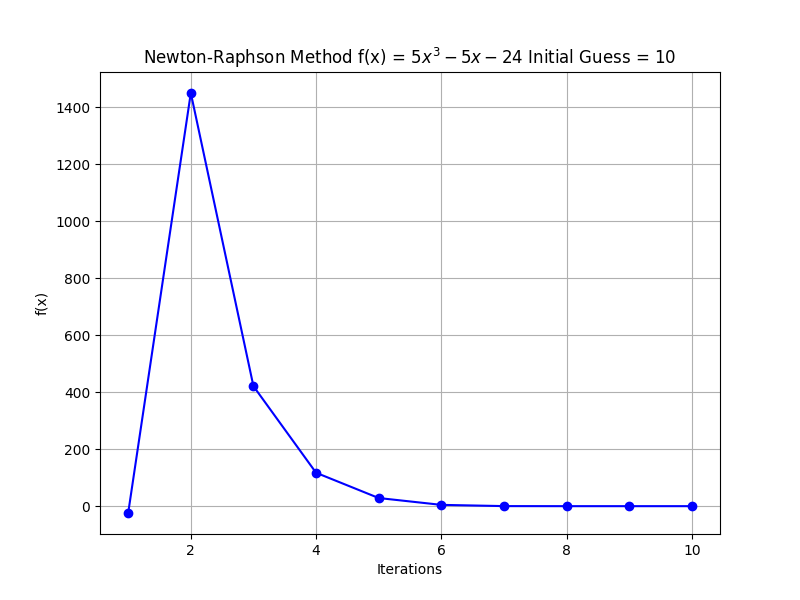
\includegraphics[width=0.8\textwidth]{../images/grafic-ex-2.2-newton-raphson-method-10.png}
                \caption{f(x) ao decorrer das itera\c{c}\~oes}
            \end{figure}
            Com o seguinte gr\'afico para o m\'etodo da secante:
            \begin{figure}[H]
                \centering
                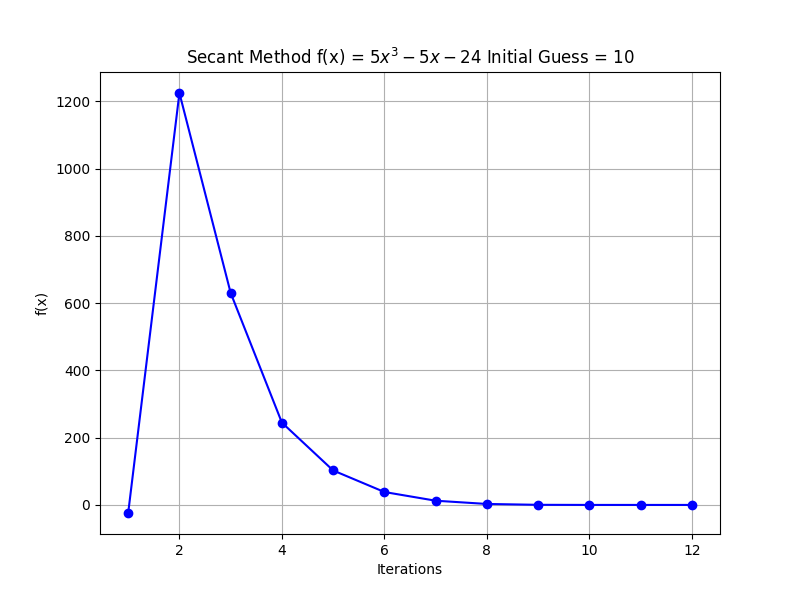
\includegraphics[width=0.8\textwidth]{../images/grafic-ex-2.2-secant-method-10.png}
                \caption{f(x) ao decorrer das itera\c{c}\~oes}
            \end{figure}

            Para as seguintes informa\c{c}\~oes iniciais:
            \begin{figure}[H]
                \centering
                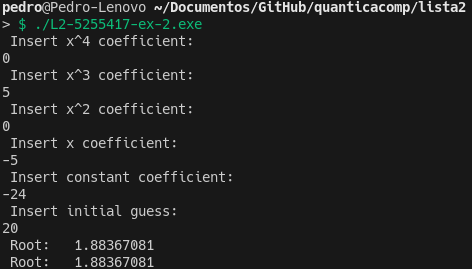
\includegraphics[width=0.8\textwidth]{../images/results-ex-2.2-20.png}
                \caption{Teste feito para gerar o gr\'afico onde as duas \'ultimas linhas s\~ao as raizes encontradas pelos m\'etodos de Newton-Raphson e da secante, respectivamente}
            \end{figure}
            Obteve-se o valor da raiz = 1.88367081 para ambos os m\'etodos.

            Com o seguinte gr\'afico para o m\'etodo de Newton-Raphson:
            \begin{figure}[H]
                \centering
                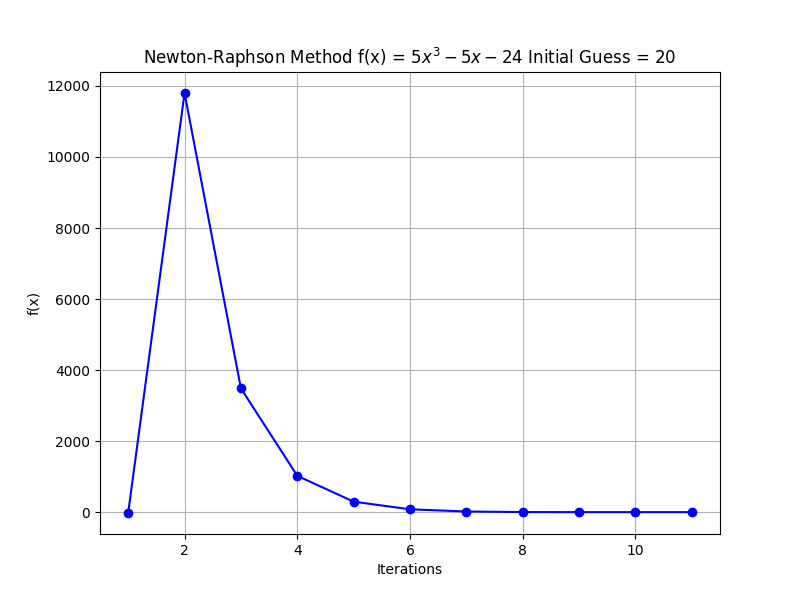
\includegraphics[width=0.8\textwidth]{../images/grafic-ex-2.2-newton-raphson-method-20.png}
                \caption{f(x) ao decorrer das itera\c{c}\~oes}
            \end{figure}
            Com o seguinte gr\'afico para o m\'etodo da secante:
            \begin{figure}[H]
                \centering
                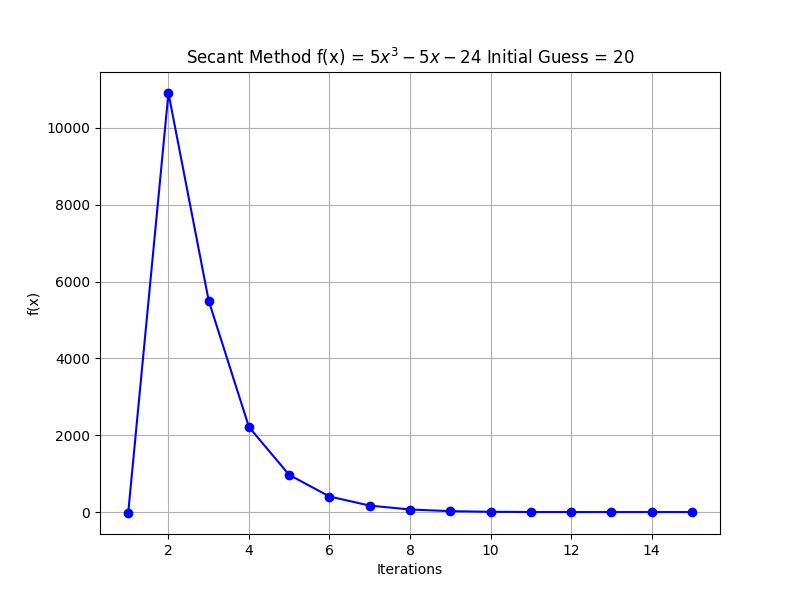
\includegraphics[width=0.8\textwidth]{../images/grafic-ex-2.2-secant-method-20.png}
                \caption{f(x) ao decorrer das itera\c{c}\~oes}
            \end{figure}

            Percebe-se que ambos os m\'etodos foram suficientes para encontrar as raizes da fun\c{c}\~ao. Contudo o m\'etodo de Newton-Raphson foi mais eficiente em encontrar em menos itera\c{c}\~oes as raizes da fun\c{c}\~ao.
            Apesar da maior efi\^encia do m\'etodo de Newton-Raphson, o m\'etodo da secante \'e \'util para casos onde a derivada da fun\c{c}\~ao \'e complicada de se calcular - ou at\'e mesmo n\~ao existe derivada.

\section{Eigenvalues of the wave equation}

    \subsection{Exerc\'icio 1}

        Tarefa: Achar a precis\~ao  do computador, i.e., o maior n\'umero positivo  tal que
        1 + $\epsilon$ = 1, usando precis\~ao simples e dupla.

        C\'odigo Escrito:
        \lstinputlisting[language=Fortran]{../L2-5255417-ex-3.f90}

        Resultados:

        Nota-se que os valores obtidos correspondem aos valores esperados.

    \subsection{Exerc\'icio 2}

        Tarefa: Calcular

        \begin{equation} e^{-x} = 1 - x + x^2/2! - x^3/3! + ... \end{equation}

        para x = 0.1, 1, 10, 100 e 1000 com um erro menor do que $10^{-8}$. Problema: quando truncar a s\'erie? \'E preciso calcular o fatorial explicitamente? Comparar o valor obtido usando a s\'erie com o resultado exato.

        C\'odigo Escrito:
        \lstinputlisting[language=Fortran]{../L2-5255417-ex-4.f90}

        Resultados:

        Descri\c{c}\~ao: O c\'odigo faz um loop onde, em cada itera\c{c}\~ao, calcula o valor da s\'erie para um valor de x diferente. Na subrotina "compute-exponencial" calcula-se a s\'erie definindo o pr\'oximo termo como a multiplica\c{c}\~ao do termo anterior por -x/n, pois - deste modo - n\~ao se faz necess\'ario calcular o fatorial explicitamente. Ademais, interrompe-se a soma quando o termo atual for menor que $10^{-8}$ garantindo a precis\~ao desejada, uma vez que cada termo da s\'erie \'e menor - em m\'odulo - que o anterior.

        Por fim, percebe-se que o resultado eperado foi obtido para todos os casos testados - com exe\c{c}\~ao dos casos onde o resultado \'e menor que a precis\~ao.

    \subsection{Exerc\'icio 3}

        Tarefa: Considerar a somat\'oria

        \begin{equation} \Sigma (N) = \sum_{n=1}^{2N} (-1)^n\frac{n}{n+1} = - \sum_{n=1}^N \frac{2n-1}{2n} + \sum_{n=1}^N \frac{2n}{2n+1} = \sum_{n=1}^N \frac{1}{2n(2n+1)} \end{equation}

        e calcular $\Sigma (N)$ para N = 1, 2, . . . , $10^6$ usando as tr\^es f\'ormulas acima. Comparar os resultados usando precis \~ao simples.

        C\'odigo Escrito:
        \lstinputlisting[language=Fortran]{../L2-5255417-ex-5.f90}

        Resultados:

        Nota-se que a primeira s\'erie demora \'e mais inst\'avel do que as demais. Al\'em disso, a terceira s\'erie se mostra mais est\'avel que a segunda - sendo ent\~ao a melhor vers\~ao.

\end{document}